\documentclass[]{article}
\usepackage{lmodern}
\usepackage{amssymb,amsmath}
\usepackage{ifxetex,ifluatex}
\usepackage{fixltx2e} % provides \textsubscript
\ifnum 0\ifxetex 1\fi\ifluatex 1\fi=0 % if pdftex
  \usepackage[T1]{fontenc}
  \usepackage[utf8]{inputenc}
\else % if luatex or xelatex
  \ifxetex
    \usepackage{mathspec}
  \else
    \usepackage{fontspec}
  \fi
  \defaultfontfeatures{Ligatures=TeX,Scale=MatchLowercase}
\fi
% use upquote if available, for straight quotes in verbatim environments
\IfFileExists{upquote.sty}{\usepackage{upquote}}{}
% use microtype if available
\IfFileExists{microtype.sty}{%
\usepackage[]{microtype}
\UseMicrotypeSet[protrusion]{basicmath} % disable protrusion for tt fonts
}{}
\PassOptionsToPackage{hyphens}{url} % url is loaded by hyperref
\usepackage[unicode=true]{hyperref}
\hypersetup{
            pdftitle={Testing session protocol},
            pdfauthor={Yiming Qian, Andrea Seisler, \& Rick Gilmore},
            pdfborder={0 0 0},
            breaklinks=true}
\urlstyle{same}  % don't use monospace font for urls
\usepackage[margin=1in]{geometry}
\usepackage{graphicx,grffile}
\makeatletter
\def\maxwidth{\ifdim\Gin@nat@width>\linewidth\linewidth\else\Gin@nat@width\fi}
\def\maxheight{\ifdim\Gin@nat@height>\textheight\textheight\else\Gin@nat@height\fi}
\makeatother
% Scale images if necessary, so that they will not overflow the page
% margins by default, and it is still possible to overwrite the defaults
% using explicit options in \includegraphics[width, height, ...]{}
\setkeys{Gin}{width=\maxwidth,height=\maxheight,keepaspectratio}
\IfFileExists{parskip.sty}{%
\usepackage{parskip}
}{% else
\setlength{\parindent}{0pt}
\setlength{\parskip}{6pt plus 2pt minus 1pt}
}
\setlength{\emergencystretch}{3em}  % prevent overfull lines
\providecommand{\tightlist}{%
  \setlength{\itemsep}{0pt}\setlength{\parskip}{0pt}}
\setcounter{secnumdepth}{0}
% Redefines (sub)paragraphs to behave more like sections
\ifx\paragraph\undefined\else
\let\oldparagraph\paragraph
\renewcommand{\paragraph}[1]{\oldparagraph{#1}\mbox{}}
\fi
\ifx\subparagraph\undefined\else
\let\oldsubparagraph\subparagraph
\renewcommand{\subparagraph}[1]{\oldsubparagraph{#1}\mbox{}}
\fi

% set default figure placement to htbp
\makeatletter
\def\fps@figure{htbp}
\makeatother


\title{Testing session protocol}
\author{Yiming Qian, Andrea Seisler, \& Rick Gilmore}
\date{2020-01-22 19:46:38}

\begin{document}
\maketitle

{
\setcounter{tocdepth}{3}
\tableofcontents
}
\subsection{Before participant
arrives}\label{before-participant-arrives}

\begin{itemize}
\tightlist
\item
  Please arrive \emph{10 minutes prior} to the participant testing time.
\item
  Check with Andrea/Yiming to see if there have been any cancellations
  or check the green folder with the daily schedule in it.
\item
  If the scheduled study is still on the books, proceed as follows.
\end{itemize}

\subsubsection{Set-up for Vision
Screening}\label{set-up-for-vision-screening}

\paragraph{Preparation}\label{preparation}

Materials for vision screening are stored on the table next to Andrea's
office.

\begin{itemize}
\tightlist
\item
  Make sure the black tape is on the floor 10ft from the HOVT Snellen
  Acuity Chart which is on the door to 503B
\item
  Place Stereo Acuity Test and Glasses on table
\item
  Place Color Vision Test on table
\item
  Place the Vision Screening Score Sheet on the table
\end{itemize}

\paragraph{Review vision screening
procedures}\label{review-vision-screening-procedures}

The vision screening protocol may be reviewed at
\href{vision-screening-protocol.html}{this link}

\subsubsection{Set up for computer-based
tasks}\label{set-up-for-computer-based-tasks}

\paragraph{Stimuli Computer}\label{stimuli-computer}

\begin{itemize}
\item
  \emph{Log into Data Collection Computer}
\item
  Turn on the power of the data collection computer
\item
  Turn on the CRT monitor in 503B
\item
  Log-in (use your indiviual PSU login)
\item
  \emph{Start Psychopy}
\item
  Click \textbf{PsychoPy} icon on Task Bar
  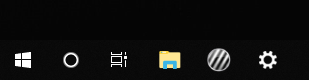
\includegraphics{images/PsychoPy-1.PNG}\\
\item
  \emph{Double-check monitor settings within Windows}
\item
  Click Settings (`gear') icon on Task Bar
  
\includegraphics{images/DispSettings-1.PNG}\\
\item
  Choose \textbf{System}\\
  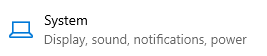
\includegraphics{images/DS2.PNG}\\
\item
  Choose \textbf{Display}\\
  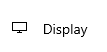
\includegraphics{images/ds3.PNG}\\
\item
  Choose \textbf{Advanced display settings} (You may need to scroll down
  to see this)\\
  
\includegraphics{images/DS4.PNG}\\
\item
  Make sure the window that appears has the following Settings\\
  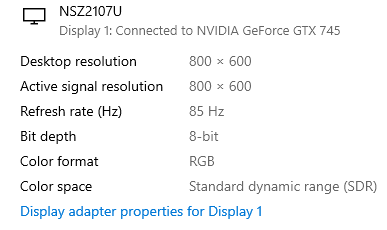
\includegraphics{images/ds5.PNG}\\
\item
  \emph{Double-check Brightness/Contrast of monitor}
\item
  Contrast:
\item
  Brightness:
\item
  Press any button on the monitor (except Signal A/B/OSD OFF and the
  Power button)
\item
  Navigate to the leftmost option in the settings menu (looks like a
  half moon)
\item
  Press the down button on the monitor
\item
  Adjust the Contrast (leftmost option) to the required setting using
  the +/- buttons on the monitor
\item
  Adjust the Brightness (second option from the left) to the required
  setting using the +/- buttons on the monitor
\item
  \emph{Check monitor within PsychoPy}\\
\item
  Go to \textbf{Monitor Settings}\\
  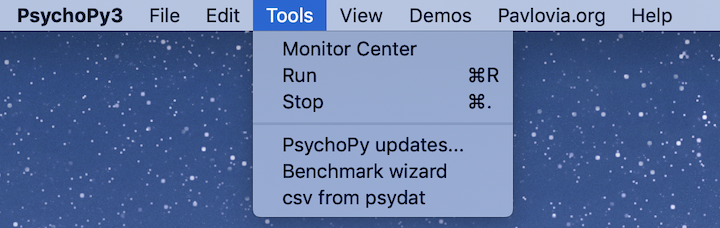
\includegraphics{images/pp2.png}\\
\item
  View Settings, they should be as follows\\
  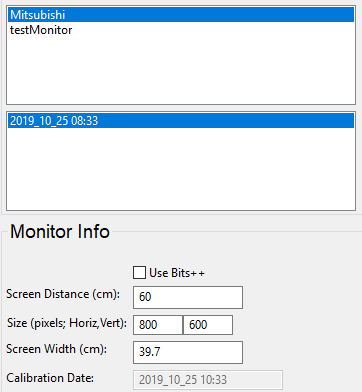
\includegraphics{images/pp3.PNG}
\end{itemize}

\paragraph{Survey Computer}\label{survey-computer}

\begin{itemize}
\tightlist
\item
  Log-in to survey computer with your individual PSU login
\item
  Load page with surveys:
  \url{https://pennstate.qualtrics.com/jfe/form/SV_5AoCVwYH7ZsXFQh}.
  \textbf{UPDATED 2019-11-18}.
\end{itemize}

\subsubsection{After participant
arrives}\label{after-participant-arrives}

\paragraph{Welcome participant}\label{welcome-participant}

Say:

\begin{quote}
``\emph{Welcome to the brain, behavior, and development lab. Are you
here for the study about individual difference of motion perception?}''
\end{quote}

Close the door. If the participant answers yes, say:

\begin{quote}
``\emph{Great. You can sit in this chair and put your coat and bags
beside you.}''
\end{quote}

\begin{itemize}
\tightlist
\item
  Store coat on back of main door and bags by the file/bookcase.
\end{itemize}

\begin{quote}
``\emph{Are you \textless{}NAME OF PERSON ON SONA SYSTEMS SITE SCHEDULED
FOR THIS SESSION\textgreater{}?}''
\end{quote}

\begin{itemize}
\tightlist
\item
  If the participant answers yes, say:
\end{itemize}

\begin{quote}
``\emph{Ok. We want to make sure that you get credit for participation.
Please sit here for the first portion of the study.}''
\end{quote}

\begin{itemize}
\tightlist
\item
  Have the person sit at the computer where the survey will be taken.
\end{itemize}

\paragraph{Begin the survey}\label{begin-the-survey}

Conduct the implied verbal consent.

\begin{quote}
``\emph{Welcome. Today you are going to participate in a set of
questionnaires, two computer visual tasks and a few vision screening
measures. Your participation is voluntary and you may decide to stop at
any time. You do not have to answer any questions that you do not want
to answer. You will receive course credit for your participation. You
may review the consent form on the screen in front of you. Do you have
any questions?}''
\end{quote}

Once the consent is complete (It means the participant clicks to the
next page), enter participant ID

\begin{itemize}
\item
  Following the consent page, there is a Participant ID blank spot on
  the top of visual acuity test page. Please use the smallest number
  available on the white board. \emph{Take a note} of this participant
  ID in ``Penn State Vision Screening Score Sheet''. Enter this number
  into the Qualtrics Survey and each of the computer tasks.
\item
  Do not choose a number before the participant arrives.
\item
  When you use a Participant ID from the white board, please cross it
  out with the brown dry erase marker. All used numbers will be erased
  at the end of the day.
\end{itemize}

Then say,

\begin{quote}
``\emph{Great. Now we'd like to move on to the first vision screening
test. Could you stand behind this line?}''
\end{quote}

\subsubsection{Complete pattern visual acuity
testing}\label{complete-pattern-visual-acuity-testing}

\subparagraph{Procedure}\label{procedure}

\begin{itemize}
\tightlist
\item
  Have participant stand 10 feet away from the chart on the wall (black
  tape on the floor)
\item
  Ask the participant to start with the top line and have the
  participant read the first symbols in every line in descending order
\end{itemize}

\begin{quote}
``Could you read the first symbols in each line for me from the top to
bottom?''
\end{quote}

\begin{itemize}
\tightlist
\item
  If they miss a letter, circle it on the score sheet.
\item
  Move back up one line and ask the participant to identify all the
  optotypes on that line. If the participant identifies all symbols
  correctly, go to the next line with smaller optotypes and ask the
  participant to identify all optotypes on the line.
\end{itemize}

\begin{quote}
``Could you read all the symbols in this line? And this line?''
\end{quote}

\begin{itemize}
\tightlist
\item
  Their visual acuity will be the one that matches the line on which
  50\% (3 of 5, 4 of 6) of the symbols are identified correctly.
\end{itemize}

\subparagraph{Report results}\label{report-results}

\begin{itemize}
\tightlist
\item
  Log the answer to each item on the
  \href{vision-screening-score-sheet.html}{score sheet}.
\item
  Log the acuity for the participant in terms of 10 ft (e.g.~10/10)
\item
  Report the result into Qualtrics
\end{itemize}

\subsubsection{Questionnaires}\label{questionnaires}

\begin{quote}
``\emph{Thank you. Now we'd like to move on to the questionnaires.
Please sit down. You can follow the instructions and finish the survey.
Feel free to ask me if you have any questions. And let me know when you
finish it.}''
\end{quote}

\begin{itemize}
\tightlist
\item
  Have the participant sit back down at the computer.
\item
  Let the participants finish the questionnaire.
\item
  Answer the questions if the participants have any, when they works on
  the questionnaires. But in careful in the hobby page, spatial and
  verbal page, because the time are recorded. The page will vanish when
  the time have passed. So, depending on the nature of the questions,
  answer them fast and emphasize the time is recorded in this page.
\end{itemize}

After answering the question, say: \textgreater{}``\emph{Beware: there
is a time limit for this page. }''

\begin{itemize}
\tightlist
\item
  If the participants have questions in the instruction page of hobby
  test, spatial and verbal test, answer careful and make sure the
  participants understand well.
\item
  After the participants finish the questionnaire, ask them if they need
  a little break. If the participant wants to keep going, lead them to
  the test room
\end{itemize}

Say:

\begin{quote}
``\emph{You have finished this part. Next you have two computer tasks.
Do you want to continue or have a little break?}''
\end{quote}

\subsubsection{Set-up for computer-based
tasks}\label{set-up-for-computer-based-tasks-1}

\begin{itemize}
\tightlist
\item
  Guide participant to the testing room.
\item
  Have them sit in the chair.
\item
  Adjust the monitor and participant position.
\item
  The monitor should be located \textbf{60cm} from the bridge of the
  nose on the participant.
\item
  \emph{place the rear legs of the chair exactly in front of black
  strips}
\item
  The chair height should be set so the participant is looking in the
  middle of the screen.
\item
  Guide the participant to use the arrow keys for responses and the
  space bar to advance the screen.
\item
  \emph{check with participants that they do not bring the cell phone to
  the dark room}
\end{itemize}

\begin{quote}
``\emph{Do you have your cell phone or is it with your bag/coat? If you
have your cell phone, please place it with your bag/coat.}''
\end{quote}

Say:

\begin{quote}
``\emph{Please come to this room for the behavioral tests. Sit in the
chair. Could I move the chair a little bit? I want to make sure every
particpant is the same distance from the computer screen. Please sit
straight and have you back touching the chair. Do not move your
chair.}''
\end{quote}

\begin{quote}
``\emph{Please do you best and focus on the center of the screen during
these tasks.}''
\end{quote}

\subsubsection{Run computer-based tasks}\label{run-computer-based-tasks}

\paragraph{Select run order}\label{select-run-order}

The order of the computer experiments will be randomized across
participants based on the participant ID entered into Qualtrics.

\begin{itemize}
\tightlist
\item
  run the \emph{temporal duration threshold task} first (Murray et al.)
  if the ID number is \emph{EVEN}.
\item
  run the \emph{contrast sensitivity task} first (Abramov et al.) if the
  ID number is \emph{ODD}. \emph{Record the task run first on the
  experiment run log.}
\end{itemize}

\paragraph{Temporal duration threshold task (Murray et
al.)}\label{temporal-duration-threshold-task-murray-et-al.}

\begin{itemize}
\tightlist
\item
  Open PsychoPy by clicking on the icon located on the desktop.
  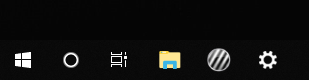
\includegraphics{images/PsychoPy-1.PNG}\\
\item
  When PsychoPy opens, open the file for this experiment.

  \begin{itemize}
  \tightlist
  \item
    From the \texttt{File} menu, select the \texttt{Open\ Recent...}
    command and select the \texttt{motion-temporal-threshold.py} file.
  \end{itemize}
\item
  When the file opens, run the experiment by pressing press the green
  (running person) button. 
\includegraphics{images/PPrunningMan.png}

  \begin{itemize}
  \tightlist
  \item
    \textbf{Be careful not to type in the programming window.}
  \end{itemize}
\item
  Experimenters need to fill in the participant ID and gender.

  \begin{itemize}
  \tightlist
  \item
    A pop-up window will appear.
  \item
    Enter participant ID. Make sure it is the same ID as that in
    qualtrics.
  \item
    Enter gender (enter ``f'' or ``m'', no upper case) in the pop
    window, and press the \texttt{Ok} button to enter the data.
  \end{itemize}
\item
  Speak to the participant
\end{itemize}

\begin{quote}
``In this task, you need to detect the moving direction of a small patch
of stripes. The time the patch appears on the display will get shorter
and shorter. Our goal is to find out the shortest duration you need to
detect the direction of motion.''
\end{quote}

\begin{quote}
``Which hand do you prefer to press the arrow keys?''
\end{quote}

\begin{quote}
``Put your fingers of your prefered hand on the left and right arrow
keys. You'll press the left arrow if you see motion to the left and the
right arrow if you see motion to the right. If you aren't sure, make
your best guess.''
\end{quote}

\begin{quote}
For the left-handed: ``You could press this ENTER key on the right side
to preceed instead of space bar.''
\end{quote}

\begin{quote}
``On the computer screen, you will see a black dot at first. When the
black dot appear, press the space bar to start the trial. Then you will
see the patch. Make responses of left or right when the white dot
appears.
\end{quote}

\begin{quote}
``Remember, accuracy is more important than speed. Please take your
time.''
\end{quote}

\begin{quote}
``Do you have any questions right now? Okay. I will leave you in the
room. Follow the instructions on the screen. Call me when you finished
this part.''
\end{quote}

\begin{itemize}
\tightlist
\item
  close the door for participants
\end{itemize}

\paragraph{Contrast sensitivity task (Abramov et
al.)}\label{contrast-sensitivity-task-abramov-et-al.}

\begin{itemize}
\tightlist
\item
  Open PsychoPy by clicking on the icon located on the desktop.
  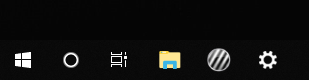
\includegraphics{images/PsychoPy-1.PNG}\\
\item
  When PsychoPy opens, open the file for this experiment.

  \begin{itemize}
  \tightlist
  \item
    From the \texttt{File} menu, select the \texttt{Open\ Recent...}
    command and select the \texttt{motion-temporal-threshold.py} file.
  \end{itemize}
\item
  When the file opens, run the experiment by pressing press the green
  (running person) button. 
\includegraphics{images/PPrunningMan.png}

  \begin{itemize}
  \tightlist
  \item
    \textbf{Be careful not to type in the programming window.}
  \end{itemize}
\item
  Experimenters need to fill in the participant ID and gender.

  \begin{itemize}
  \tightlist
  \item
    A pop-up window will appear.
  \item
    Enter participant ID. Make sure it is the same ID as that in
    qualtrics.
  \item
    Enter gender (enter ``f'' or ``m'', no upper case) in the pop
    window, and press the \texttt{Ok} button to enter the data.
  \end{itemize}
\item
  Speak to the participant
\end{itemize}

\begin{quote}
``You will see a small patch of black and white stripes which is
horizontal or vertical.Be careful. You need to detect the direction of
the stripes not the moving direction. (Show her the example pictures put
in the left side of desk). You can press the LEFT key if you see the
stripes are horizontal, DOWN key if you see the stripes are vertical.
But if you aren't sure, just guess.''
\end{quote}

\begin{quote}
``The luminance of the stripes will get smaller and smaller. Our goal is
to find out the smallest luminance that you need to detect the direction
of stripes.''
\end{quote}

\begin{quote}
``Which hand do you prefer to press the arrow keys?''
\end{quote}

\begin{quote}
``Put your fingers of your prefered hand on the left and down keys.
You'll press the left key if you see see horizontal stripes and the down
key if you see vertical stripes. If you aren't sure, make your best
guess.''
\end{quote}

\begin{quote}
For the left-handed: ``You could press this ENTER key on the right side
to preceed instead of space bar.''
\end{quote}

\begin{quote}
``Remember, accuracy is more important than speed. Please take your
time.''
\end{quote}

\begin{quote}
``Do you have any questions right now? Okay. I will leave you in the
room. Follow the instructions on the screen. Call me when you finish
this part.''
\end{quote}

\begin{itemize}
\tightlist
\item
  close the door for participants
\end{itemize}

\subsubsection{Stereo acuity and color vision
tests}\label{stereo-acuity-and-color-vision-tests}

\begin{quote}
``\emph{Thank you so much. We are going to complete two more short
vision tests. Please come sit over here at this table.}''
\end{quote}

Escort participant to table.

\paragraph{Color Test}\label{color-test}

\subparagraph{Procedure}\label{procedure-1}

\begin{itemize}
\tightlist
\item
  The examination should be done indoors with bright, natural
  illumination of more than 300 lux.
\item
  The plates should be held at a distance of 50 - 75 cm (20-30 inches)
\end{itemize}

Say:

\begin{quote}
``This test assesses your color vision. Look at this picture and tell me
what you see.'' ``Now trace the curve.''
\end{quote}

\begin{itemize}
\tightlist
\item
  The first exam:

  \begin{itemize}
  \tightlist
  \item
    *Skip: Examiner shows the participant plate 1 or 2, tracing the red
    line. Recognized as ``circle'', ``square'', or some other design.
  \item
    Plate 3 and 4. The participants are required to say outloud
    ``circle'', ``square'', or some other design. If the shape is
    correctly recognized, mark as normal.If the shape is not correctly
    recognized, mark as abnormal.
  \end{itemize}
\item
  The second exam:

  \begin{itemize}
  \tightlist
  \item
    Skip: Examiner shows the participant plate 5. Recognized as a curve
    line.
  \item
    Plate 6: In tracing the winding line between the upper left mark x
    and lower right mark x, the normal traces the red curve, but the
    abnormal usually trace the blue.
  \item
    Plate 7: In tracing the winding line between the upper left mark x
    and lower right mark x, the normal traces the upper green curve, but
    the abnormal usually trace the lower red curve.
  \item
    Plate 8: In tracing the winding line between the upper left mark x,
    the normal can trace upper and lower curve and come back to the
    starting mark. In case of abnormal color vision, some can trace
    either contour.
  \end{itemize}
\end{itemize}

When the participant is finished, say:

\begin{quote}
``Great. Thank you.''
\end{quote}

\subparagraph{Report results}\label{report-results-1}

\begin{itemize}
\tightlist
\item
  Log the answer to each item on the score
  \href{vision-screening-score-sheet.html}{score sheet}.
\item
  Those who can not recognize any curve in plate 8 at all, or any lower
  curve are definitely abnormal.
\item
  They might be abnormal if they misjudge more than 3 plates among
  plates 3,4,6,7
\item
  If they misjudge 1-2 plates among plates 3,4,6,7, it is better to
  re-examine him in details from plate 1-8.
\item
  Report the result into Qualtrics
\end{itemize}

\paragraph{Stereo Vision Test}\label{stereo-vision-test}

\subparagraph{Procedure}\label{procedure-2}

\begin{itemize}
\tightlist
\item
  Have the participant put the stereo glasses on.
\item
  Provide good light, make sure the pictures maintain the proper axis of
  polarization before the participants at 15 minutes of arc at a
  distance of 16 inches.
\item
  Only do the circle test. Point to each item on the left hand side of
  the page going left to right and up to down.
\item
  Start with No.1.
\end{itemize}

Say:

\begin{quote}
``\emph{This test assesses your stereoacuity. Do you see the butterfly?
Look at each of the four circles and tell me which one seems to come out
closer to you-top, bottom, right, or left.}''
\end{quote}

Continue until participant gives up trying, or making two successive
mistakes. - Some participants may develop this perceptual response
slowly. So let them study it for a while or let them change the viewing
angle, if needed.

\subparagraph{Report results}\label{report-results-2}

\begin{itemize}
\tightlist
\item
  Log the answer to each item on the
  \href{vision-screening-score-sheet.html}{score sheet}.
\item
  Record the level of stereopsis into Qualtrics at the last one chosen
  correctly.
\end{itemize}

\subsection{After session ends}\label{after-session-ends}

\subsubsection{Thank participant}\label{thank-participant}

\begin{itemize}
\tightlist
\item
  After the participant finishes all the tests, thank him/her.
\end{itemize}

\begin{quote}
``\emph{These are all the tasks for today. Thank you for participation.
We appreciate your time. Do you have any questions?}''
\end{quote}

\begin{itemize}
\tightlist
\item
  Answer any questions the participant might have. You may direct them
  to Yiming or to Dr.~Gilmore if you are unable to answer the question.
\item
  If the participant ask the purpose of this study, read the debrief
\end{itemize}

\paragraph{debrief}\label{debrief}

``In this study, the visual scuity test, color vision test and stereo
vision test are conducted to make sure you have normal vision to detect
the motion in short period or low luminance.

You also have done two computer tests, which examine your performance in
motion perception. In this study, we want to investigate whether or how
motion perception is correlated with individual's verbal ability,
spatial ability, or personal interests. "

\begin{quote}
``\emph{Okay. The principal investigator will give you the credit by the
end of the next business day.}''
\end{quote}

\begin{itemize}
\tightlist
\item
  Say bye to participants
\end{itemize}

\subsubsection{Give participant credit on
SONA}\label{give-participant-credit-on-sona}

\begin{itemize}
\tightlist
\item
  Yiming or Andrea will assign credit in SONA.
\end{itemize}

\subsubsection{Clean-up}\label{clean-up}

\begin{itemize}
\tightlist
\item
  Mark on the daily schedule sheet in the green folder if:

  \begin{itemize}
  \tightlist
  \item
    the participant was Present or a No Show\\
  \item
    the number used for that participant if Present
  \end{itemize}
\item
  Clean keyboard, mouse and table and begin
  \href{sex-differences-data-export.md}{data export} (separate
  protocols).
\end{itemize}

For the last participant of the day: - Copy the data of this participant
to the hard drive

\end{document}
